\documentclass[conference]{IEEEtran}
\IEEEoverridecommandlockouts
% The preceding line is only needed to identify funding in the first footnote. If that is unneeded, please comment it out.
\usepackage{cite}
\usepackage{amsmath,amssymb,amsfonts}
\usepackage{float}
\usepackage{algorithm, algorithmic}
\usepackage{graphicx}
\usepackage{booktabs}
\usepackage{textcomp}
\usepackage{xcolor}

\def\BibTeX{{\rm B\kern-.05em{\sc i\kern-.025em b}\kern-.08em
		T\kern-.167em\lower.7ex\hbox{E}\kern-.125emX}}
	
\newtheorem{theorem}{Theorem}[section]
\newtheorem{corollary}{Corollary}[theorem]
\newtheorem{lemma}[theorem]{Lemma}
\newtheorem{example}[theorem]{Example}
\begin{document}
	
	\title{A Method For Listing All Low-Weight Parity Bit Codewords For RSC Codes\\
	}
	
	\author{
		\IEEEauthorblockN{1\textsuperscript{st} Bohulu Kwame Ackah}
		\IEEEauthorblockA{\textit{Graduate School of Informatics and Engineering} \\
			\textit{The University of Electro-Communication}\\
			Tokyo, Japan \\
			bohulu@uec.ac.jp}
		\and
		\IEEEauthorblockN{2\textsuperscript{nd} Chenggao Han}
		\IEEEauthorblockA{\textit{Department of Communication Engineering and Informatics} \\
			\textit{The University of Electro-Communication}\\
			Tokyo, Japan \\
			han.ic@uec.ac.jp}
	}
	
	\maketitle
	
	\begin{abstract}
In this paper, we present a novel method for listing all message inputs which produce codewords with low-weight parity bit sequences for a for a given $(n,k)$ Recursive Systematic Convolutional (RSC) Code.
This method involves treating  the RSC code as closed finite-state machine and determining all paths through the trellis that begin and end at state 0 for a given trellis length $N$. Using this method, we determine all messages which produce codewords with parity-bit sequence weight $W_p=2$ and $W_p=4$ for $N=64$. We calculate the upper-bound for the Probability of Bit Error  of the given RSC code using the partial distance spectrum obtained using the proposed method. Simulation results reveal that this new bound is either tighter than or very close to existing  bounding techniques.
\end{abstract}

	
	\linespread{2.0}	
\section{Introduction}

A Convolutional Code(CC) is generated by passing a message input through a linear finite-state shift register. The structure of this code is such that it is best described using a trellis. This structure makes it possible to employ soft decision decoding algorithms, the most popular of these algorithms being the Viterbi algorithm. CC are used extensively in mobile communication and space communication application as a major component in concatenated code.  Depending on the configuration of the shift register being used to generate the code, a CC can either be \textit{recursive} or \textit{nonrecursive}. In the case of the recursive CC, a feedback shift register is used to generate the code. Furthermore if the the message input appears in the CC, it is known as \textit{systematic}. Recursive Sytematic Convolutional Codes(RSCC's) are used as component codes for Turbo codes, which are one of the few error correcting codes with performance very close to the Shannon limit[1].

Low weight codeword may be produced when the parity bit sequence has a very low weight. Amongst all such codewords, the one with the lowest weight determines the free distance $d_{\text{free}}$ of the code. 
$d_{\text{free}}$  of a RSCC is a very important factor and determines its error-correction performance[4].  This can be obtained from the distance spectrum of the RSCC. This can be found from the transfer function $T(D,N)$ , where 
$$
T(D,N)=\sum_{i=0}^{\infty}\sum_{d=0}^{\infty} a(d,i)D^dN^i
$$

and $a(d,i)$ is the number of codewords present in the code with weight $d$ that were generated by a message input of weight $i$. $D ~\text{and} ~ N$ are dummy variables [3]. As the number of states present in the RSCC increases so does the complexity involved in calculating the transfer function. Furthermore, the transfer function only provides information about the number of codewords of weight $d$ generated by message input of weight $i$. There is no extra information with regards to the structure of the message input which generates which low-weight parity bit sequences and possibly low-weight codewords.

In this research paper, we present a novel method which can be used to easily determine which message inputs of length $N$ will result in parity bit sequences of weight $W_p$ after it has been encoded with an RSC encoder. This method does not require the calculation of the transfer function of the RSCC. Using this method we calculate the theoretical upper bound for the given RSC code using the partial distance spectrum obtained. The rest of the research paper is organised as follows. In Section \ref{sec2}, we give a brief review of RSC codes. In section Section \ref{sec3}, we present our novel method and in section \ref{sec4}, we derive the upper bound for a given RSC code based on our novel method. Simulation results are presented in Section \ref{sec5} and we conclude our research paper and discuss future works in Section \ref{sec6}

\section{Recursive Systematic Convolutional Codes:Review}
\label{sec2}

An  $(n,k)$ RSCC is a convolutional code generated by using feedback shicft registers which has its input bits as part of the codeword. At each time instant it receives an input of $k$ bits and outputs $n$ bits. The output bits are determined by the generator function, which may be written in $D$ notation as  $[1 ~\frac{F(D)}{H(D)}]$ or simply as $[\frac{F(D)}{H(D)}]$ where $F(D)$ and $H(D)$ represent the feedfoward and feedback connections of the component encoder.

It should be noted that the prescence of the feedback loop means that the code procuded will have an infinite-length impulse response. A parameter which arises as a result of this infinite impulse response is know as the cycle length which we will represent by $\tau$. The cycle length is defined as the output cycle of an RSC encoder when the input is $(1 0 0 0 .....)$[5]. This output which is represented by $\textbf{t} $ is with respect to the parity check bits only and is the impulse response of the RSCC. The cycle is represented by $\textbf{p}$ and is unique for each RSCC. 

%To improve the ability of a decoder, it is requred that the start state and the end state be the same. The process of doing this is know as \textit{terminating} the code. Popular methods include tail-biting and terminating with extra bits. In all our simulations both methods are employed.

For the decoding of RSCC's, the Viterbi decoder is used. The idea is to go through the trellis of the RSCC and determine the most probable path throught the trellis which corresponds to the transmitted message input. For a RSCC some message inputs are more prone to being decoded wrongly than others. These usually correspond to messages which produce low weight parity bits. 

\begin{figure}[h]
\centering
		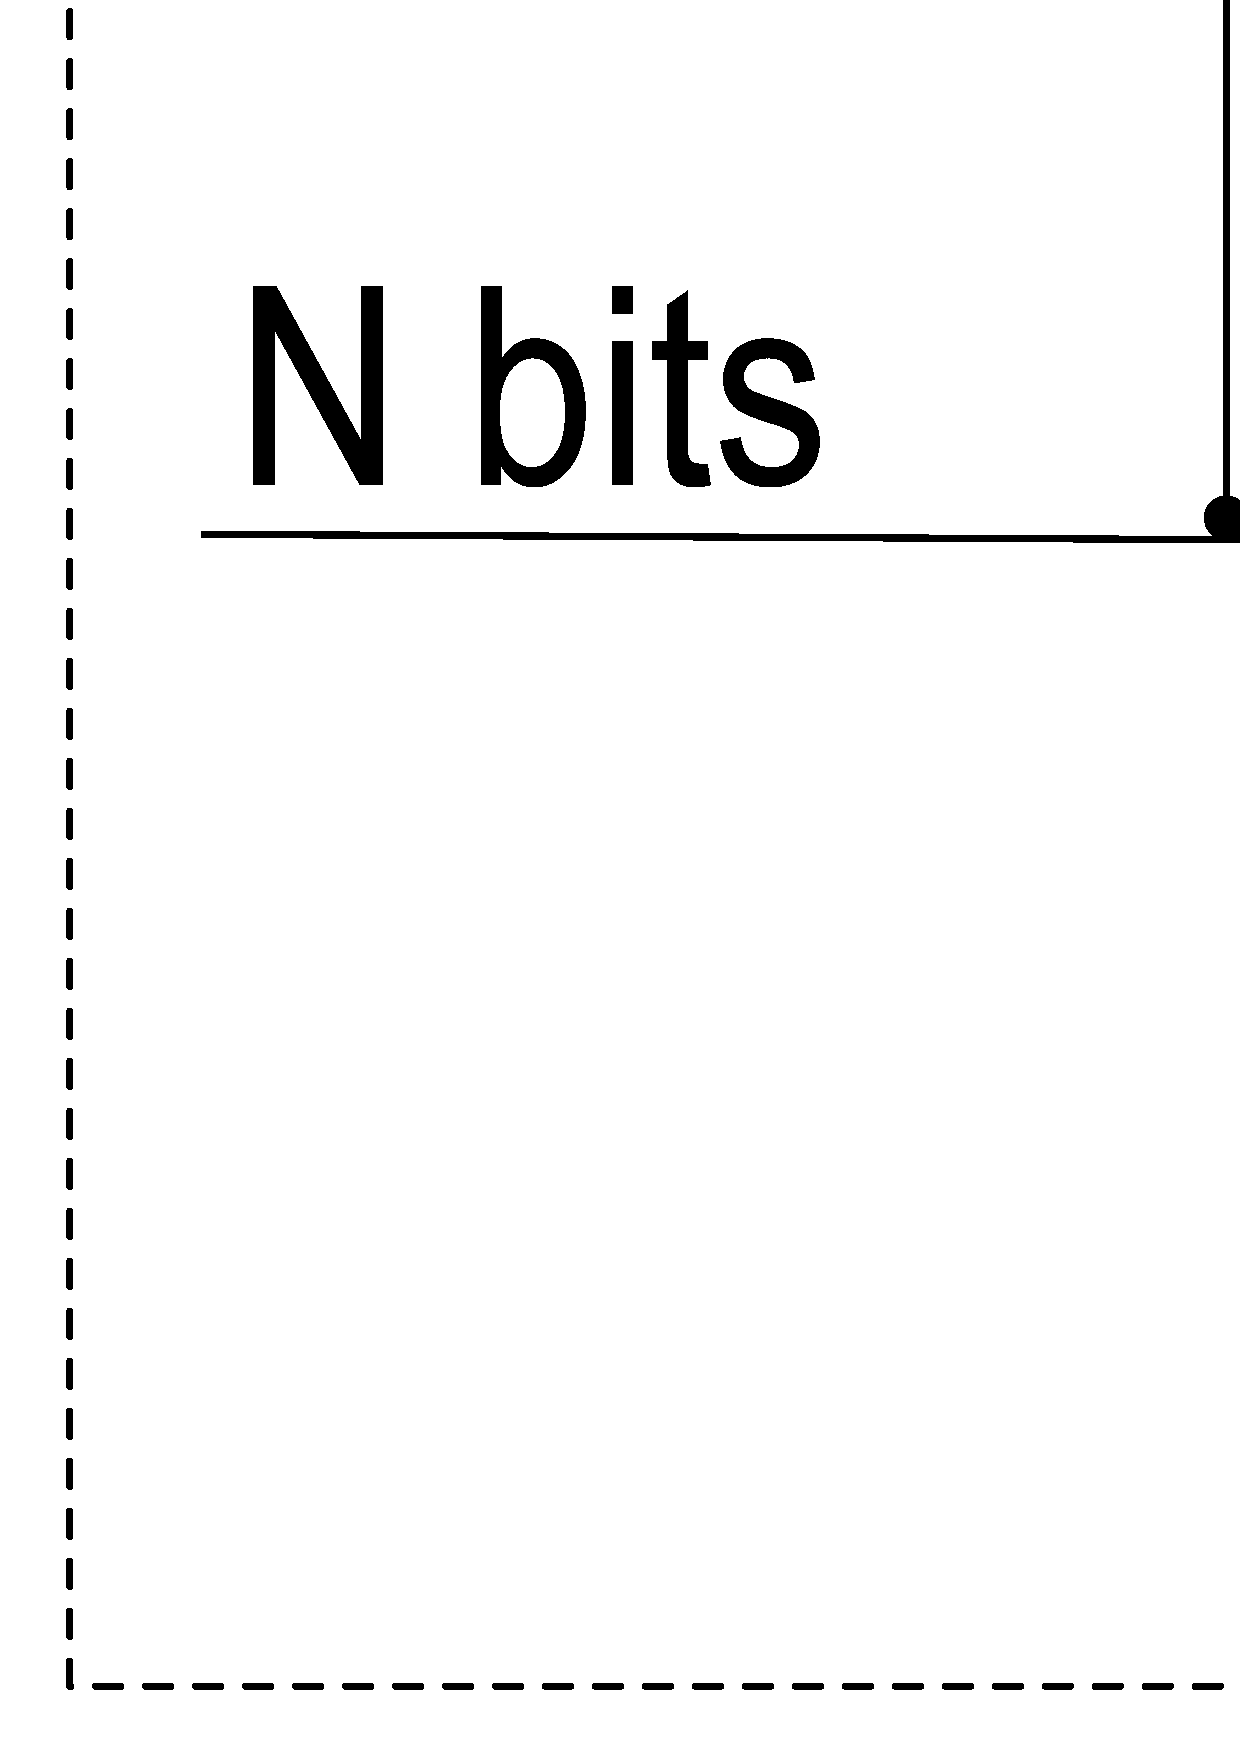
\includegraphics[width=0.45\textwidth]{RSCExample3.pdf}
		\caption{$[\frac{1+D^2}{1+D+D^2}]$  RSC Encoder}
		\label{fig1}
		\end{figure}
		
An RSC encoder is shown in Figure \ref{fig1}. Its generator function is given by $[\frac{1+D^2}{1+D+D^2}]$ which may be written as $(5,7)$ in octal form where $5 ~ \text{and} ~ 7$ correspond to the numerator and denomenator of the generator function respectively. 
 For the $(5,7)$ RSC code, the output is of the form $\textbf{t}=[1 1 1 0 1 1 0 1 1 0 ...]$ which gives us a cycle $\textbf{p}$ of $[1 1 0]$ and a cycle length $\tau =3$.
The knowledge of $\textbf{p}$ and $\tau$ will be used in deriving the method for determing which input messages generate low-weight parity bits. 


\section{Method for Determining Parity Check Bit Weights}
\label{sec3}
In this section, we wish to present a method for determining the input messages which generate low weight parity bits.

 \begin{table*}[h!]
 
 \caption{codewords with parity bit sequence weight $w_H(\textbf{c})=2$}
\centering
 \begin{tabular}{c c c c} 
 \hline
 $w_H(\textbf{b})$ & $a(x)$ & $b(x)$ & $c(x)$ \\ [0.5ex] 
 \hline\hline
 3 & 1 & $1+x+x^2$ & $1+x^2$\\ 
 4 & $1+x^2$ & $1+x+x^3+x^4$ & $1+x^4$ \\
 5 & $1+x^2+x^4$& $1+x+x^3+x^5+x^6$ & $1+x^6$ \\
 6 & $1+x^2+x^4+x^6$& $1+x+x^3+x^5+x^7+x^8$& $1+x^8$ \\
 7 & $1+x^2+x^4+x^6 +x^8$ & $1+x+x^3+x^5+x^7+x^9+x^{10}$ & $1+x^{10}$ \\
 8 & $1+x^2+x^4+x^6 +x^8 +x^{10}$ & $1+x+x^3+x^5+x^7+x^9+x^{11}+x^{12}$ & $1+x^{12}$\\ 
 9 & $1+x^2+x^4+x^6 +x^8+x^{10}+x^{12}$ & $1+x+x^3+x^5+x^7+x^9+x^{11}+x^{13}+x^{14}$ & $1+x^{14}$ \\ [1ex] 
 \hline
 \end{tabular}
 \label{tab1}
\end{table*}


%$b(x) = b_0x^0+b_1x_1+...+b_{N-1}x_{N-1}$ 
Let $\textbf{b} =[b_0 b_1 ... b_{N-1}]$ be a message input of length $N$ . We assume that $\textbf{b}$ is encoded using the $(5,7)$ RSC encoder to produce a codeword $\textbf{v}=[v_0 v_1 v_2 v_3 v_4 v_5 ... v_{2N-1}]$. This codeword is formed from multiplexing  systematic bits and the parity bits. The systematic bits are made up of the message input itself and are found in the even numbered part of the codeword, whiles the parity bits are determined by the past and present input bits fed into the encoder. 
We represent the parity bits by 
$\textbf{c}=[c_0 c_1 c_2 ... c_{N-1}] \equiv [v_1 v_3 v_5 ... v_{2N-1}]$

As mentioned earlier,our interest is to determine if a given message input $\textbf{b}$ will produce low-weight parity bit sequence. With the knowlege of the impulse response of the  RSC encoder and a little algebra, it is possible to determine what the parity bits will be and by extension, the weight of the parity bits. 
 
 We write $\textbf{b}$ and $\textbf{c}$ in polynomial form as $b(x)$ and $c(x)$. We also represent the impulse in polynomial form as $t(x)$. In the polynomial representation, only ``1'' bits are of interest. Also all calculations are carried out using modulo 2 arithmetic.
$c(x)$ is calculated using (\ref{eq3})
 \begin{equation}
 \begin{split}
 c(x)&=\hat{t}(x)b(x)\\
 \end{split}
 \label{eq3}
 \end{equation}
 where $\hat{t}(x)$ is $t(x)$ written ignoring all powers greater than $x^{\tau}$
 
 We focus on the portion of $c(x)$ with powers greater than $x^{(n)}$ , where $n$ is the highest power of b(x). We refer to it as the stational state and represent it in polynomial form as $c_p(x)$.  We may write $c_p(x)$ using equation 

 \begin{equation}
 c_p(x)  \equiv b(x)p(x) ~\mod{ 1+ x^{\tau}}\\
 \label{eq1}
 \end{equation}
where $p(x)$ is the cycle $\textbf{p}$ of the  RSC code in polynomial form.
 
 in the case where $c_p(x) = 0$ ,c(x) will have a low weight.  We may write $b(x)$ as 
 $$b(x) \equiv  0_{\tau}(x) ~\mod{ g(x)} $$ which means  it is possible to factorize $b(x)$ as 
 %$b(x) \equiv  0_{\tau}(x) ~\mod{ g(x)} $ 
 \begin{equation}
 b(x) =g(x)a(x)
 \label{eq2}
 \end{equation}
 where $a(x)$ is the quotient obtained after dividing $c_p(x)$ by $1+ x^{\tau}$
 
 Given $b(x)$ and $a(x)$, it is possible to calculate $g(x)$ via polynomial division.
 
 Fixing (\ref{eq2}) into (\ref{eq3}) we have 
 
 \begin{equation}
 \begin{split}
 c(x)&=\hat{t}(x)b(x)\\
 &=\hat{t}(x)g(x)a(x)\\
 & = h(x)a(x)
 \end{split}
 \label{eq4}
 \end{equation}
 where  $h(x)=\hat{i}(x)g(x)$ 
 
 The process is explained further in Example  \ref{ex1}  and Example  \ref{ex1} for $\textbf{b}^{(0)}=[ 0 0 0 0 1 1 1 0 0 0 0 0 0 0 0 0]$ and  $\textbf{b}^{(1)}=[ 1 0 1 0 0 0 0 0 0 0 0 0 0 0 0 0 ]$ for the $(5,7)$ RSC encoder. The impulse response $t(x)=1+x+x^2+x^4+x^5+x^7+x^8+....~,p(x)=1+x ~ \text{and} ~ \hat{t}(x)=1+x+x^2$
 
  %In the case of the $(5,7)$ RSC code $\hat{i(x)}=1+x+x^2$ and therefore $h(x)=(1+x+ x^{2})(1+x+ x^{2}) = 1+x^2+ x^4 =1+x^2$ since everything from$ x^4$ is zero when $b(x) \equiv  0_{\tau}(x) ~\mod{ 1+x+ x^{2}} $
\begin{example}
\label{ex1}
$\textbf{b}^{(0)}=[ 0 0 0 0 1 1 1 0 0 0 0 0 0 0 0 0],~b^{(0)}(x)=x^4+x^5+x^6$

\begin{enumerate}
\item Determine if $c_p^{(0)}(x) =0(x)$

\begin{equation*}
\begin{split}
c_p^{(0)}(x)& \equiv b^{(0)}(x)p(x) \mod{1+x^{\tau}}\\
& \equiv (x^4+x^5+x^6)(1+x)  \mod{1+x^{3}}\\
&\equiv x^4+x^7  \mod{1+x^{3}} =0(x) ~\text{with remainder }~ a(x) =x^4
\end{split}
\end{equation*}

\item Find $g(x)$
 
 \begin{equation*}
 \begin{split}
 b^{(0)}(x)&=g(x)a(x) \\
 g(x) &=\frac{b^{(0)}(x)}{a(x)}\\
 &=\frac{x^4+x^5+x^6}{x^4}\\
 &=1+x+x^2
 \end{split}
 \end{equation*}
 
 \item Find $c^{(0)}(x)$
 \begin{equation*}
 \begin{split}
 c^{(0)}(x)&=\hat{i}(x)g(x)a(x) \\
 &=(1+x+x^2)^2(x^4)\\
 &=x^4+x^6 ~\text{and}~ h(x)=1+x^2 
 \end{split}
 \end{equation*}
 
\end{enumerate}
\end{example}

\begin{example}
\label{ex2}
$\textbf{b}^{(1)}=[ 1 0 1 0 0 0 0 0 0 0 0 0 0 0 0 0 ],~ b(x)=1+x^2$

\begin{enumerate}
\item Determine if $c_p^{(1)}(x) =0$

\begin{equation*}
\begin{split}
c_p^{(0)}(x)& \equiv b^{(1)}(x)p(x) \mod{1+x^{\tau}}\\
& \equiv (1+x^2)(1+x)  \mod{1+x^{3}}\\
&\equiv 1+x+x^2+x^3  \mod{1+x^{3}}\\ &=x+x^2 \neq 0
\end{split}
\end{equation*}
\end{enumerate}
\end{example}
 
 With this knowledge, it is possible to find all message inputs which produce low-weight parity bit sequences and by extension all codewords  with low-weight parity bits. Applying this method directly requires testing all message inputs of length $N$ which is time-consuming and very inefficeint. A better method will be to find all values of $a(x)$ which produce $c(x)$, where $c(x)$ has a low parity weight. This can be acheived using the finite state configuration shown in Figure \ref{fig2}. The state table is shown in Table \ref{tab3}. 
 
\begin{figure}[h]
\centering
		\includegraphics[width=0.45\textwidth]{fsm.png}
		\caption{Finite State Machine Configuration}
		\label{fig2}
		\end{figure}
		
		
		\begin{table*}[h!]
 
 \caption{codewords with parity bit sequence weight $w_H(\textbf{c})=4$}
\centering
 \begin{tabular}{c c c c} 
 \hline
 $w_H(\textbf{b})$ & $a(x)$ & $b(x)$ & $c(x)$ \\ [0.5ex] 
 \hline\hline
 2 & 1+x & $1+x^3$ & $1+x+x^2+x^4$\\ 
 \hline 
  & $1+x+x^2$& $1+x^2+x^4$& $1+x+x^3+x^4$ \\
   3 & $1+x+x^3$& $1+x^4+x^5$ & $1+x+x^2+x^5$ \\
  & $1+x^2+x^3$ & $1+x+x^5$ & $1+x^3+x^4+x^5$ \\
  \hline 
  & $1+x+x^2+x^3 $ & $1+x^2+x^3+x^5$ & $1+x+x^4+x^5$ \\
  & $1+x+x^2+x^4 $ & $1+x^2+x^5+x^6$ & $1+x+x^3+x^6$ \\
 4 & $1+x+x^3+x^5 $ & $1+x^4+x^6+x^7$ & $1+x+x^2+x^7$\\ 
  & $1+x^2+x^3+x^4 $ & $1+x+x^4+x^6$ & $1+x^{3}+x^5+x^6$ \\ 
  & $1+x^2+x^3+x^5 $ & $1+x+x^6+x^7$ & $1+x^{3}+x^4+x^7$ \\  
  & $1+x^2+x^4+x^5 $ & $1+x+x^3+x^7$ & $1+x^5+x^6+x^7$ \\ 
 [1ex]
 \hline
 \end{tabular}
 \label{tab2}
\end{table*}
		The trellis length is set to $N$ and initial state is set to all-zero and the initial input into finite-state machine are set to $1$.  We trace all paths throught the trellis which begin and end at the all-zero state at a stage N of the trellis. $a(x)$ corresponds to the inputs which produce such paths and $b(x)$ corresponds to outputs produced by such paths. Once all valid paths are found we can calculate $g(x)$ using (\ref{eq4}) . Finally, we can find all corresponding values of $b(x)$ using (\ref{eq3}).
 
 For $N=16$ we find all $b(x) ~\text{and}~ c(x)$ for which $w_H(\textbf{c})=2 ~\text{and} ~ w_H(\textbf{c})=4$. The results are shown in Table \ref{tab1} and \ref{tab2} respectively . For $w_H(\textbf{c})=4$, only the first 10 results are shown.  
 
   \begin{table}[h!]
 
 \caption{State Table for Finite State Machine in Fig. \ref{fig2}}
\centering
 \begin{tabular}{c c c c} 
 \hline
 $a(x)$ & S & $S'$ & $c(x)$ \\ [0.5ex] 
 \hline\hline
 0 & $0 0 $& $0 0$ & $0$\\ 
  1& $0 0$ & $1 0$ & $1$ \\
  0 & $0 1$& $0 0$ & $1$ \\
  1& $0 1$& $1 0$& $0$ \\
  0& $1 0$ & $0 1$ & $0$ \\
 1 & $1 0 $ & $1 1$ & $1$\\ 
 0 & $1 1$ & $0 1$ & $1$ \\ 
 1 & $1 1$ & $1 1$ & $0$ \\ [1ex] 
 \hline
 \end{tabular}
 \label{tab3}
\end{table}
 
  For each stage in the trellis, the number of paths through the trellis is squared. To reduce the number of calculations per stage, we calculate the weight of the path and get rid of all paths that have an output weight greater than a target weight $w_H(\textbf{c})$
 
\section{Upper Bound for RSC codes}
\label{sec4}
After a message input \textbf{b} is encoded, it is modulated using an appropriate modulation scheme and transmitted to the receiver over a channel. If the channel is AWGN, noise is added to the signal and the signal at the receiver is $\textbf{r}=[r_0,r_1,r_{2N-1}]$. The receiver demodulates the signal and uses appropriate decoding and detection schemes to produce an estimate of \textbf{b}, $\hat{ \textbf{b} }$. If a wrong decision is made, we say that an error has occurred. To measure how efficient a code is at correcting errors the Bit Error Rate (BER) is used. In most cases, the BER for a code not easily determined and bounds are calculated to give an idea as to how efficient the code is at correcting errors. There are a number of equations used to calculate the upper bound for the BER of a CC and these equations also apply to RSCC. For the case where the code is BPSK modulated and soft Viterbi decoding algorithm is used, the probability of bit error $P_b$ can be calculated using the equation below[3].

\begin{equation}
P_b \leq \frac{1}{k} \sum_{d=d_{\text{free}}}^{\infty} w(d) Q\Bigg( \sqrt{\frac{2dE_c}{N_0}}\Bigg)
\label{eq5}
\end{equation}
where $w(d)=\sum_{i=1}^{\infty} i~ a(d,i)$, $E_c/N_0$ is the Signal to Noise ratio for the transmitted codeword and $d_{\text{free}}$ is the free distance of the code. This equation require the knowledge of the distance spectrum of the RSCC and as N increases so does the number of computations required to find $w(d)$. For this reason, calculation of $w(d)$ is limited to the first few terms of the distance spectrum. 

Using the method described in the previous section, it is possible to obtain a partial distance spectrum and this partial distance spectrum can be used with (\ref{eq5}) to calculate the upper bound of the RSCC. 

By applying a bound on the Q function of the form $$Q(\sqrt{x+y}) \leq Q(\sqrt{x})e^{-y/2}$$ we obtain another bound for calculation $P_b$ as shown in (\ref{eq6}).

\begin{equation}
P_b \leq  \frac{1}{k} e^{d_{\text{free}}E_c/N_0}Q\Bigg( \sqrt{\frac{2d_{\text{free}}E_c}{N_0}}\Bigg) \frac{\partial T(D,N)}{\partial N}\Bigr|_{\substack{N=1,~D=e^{-E_c/N_0}}}
\label{eq6}
\end{equation}

Where  $T(D,N)$ is the transfer function of the RSC code. 

We obtain the partial distance spectrum for all input messages $b(x)$ of length $N=64$ which produce low-weight parity bits
$c(x)$ where $w_H(\textbf{c})=2 ~\text{and} ~ w_H(\textbf{c})=4$. We then use those terms to calculate the probability of bit error using (\ref{eq5}). We then compare it to the upper bound in (\ref{eq6}) as well as the simulation results obtained for the $(5,7)$ RSC encoder
\section{Simulation Results}
\label{sec5}

\begin{figure}[h]
\centering
		\includegraphics[width=0.45\textwidth]{paperg2.png}
		\caption{Simulation and Upper Bounds for $(5,7)$ RSCC}
		\label{fig3}
		\end{figure}
		
		The simulation results as well as the upper bounds calculated using (\ref{eq5}) and (\ref{eq6}) are shown in Figure \ref{fig3}. 
		For the $(5,7)$ RSC encoder, $d_{\text{free}}=5$, $$\frac{\partial T(D,N)}{\partial N} =\frac{D^5N^2(N-DN^2+D)}{1-2D(N-DN^2+D)}$$ and $$\frac{\partial T(D,N)}{\partial N}\Bigr|_{\substack{N=1}} = \frac{3(D-1)^2D^5}{(1-2D)^2}$$
		The old bound is calculated using  (\ref{eq5}) whiles the new bound is calculated using  (\ref{eq6}). For the simulation, $N=64$ and the soft-Viterbi algorithm is used. Also we use a tail-biting trellis structure is used. As can be seen from Figure \ref{fig3} the new bound provides a tighter bound compared to that of the older bound, especially in the higher $E_b/N_0$ region.
\section{Conclusion and Future Works}
\label{sec6}
In this research paper, we presented a method for listing all message inputs which produce codewords with low-weight parity bit sequences for a for a given $(n,k)$ Recursive Systematic Convolutional (RSC) Code. Using a specially configured finite state machine, we were able to obtain a partial distance spectrum which we use to calculate an upper bound for the RSCC. Through simulation, we are able to confirm that the new bound is tighter than existing ones. 




\begin{thebibliography}{99}
\bibitem{ref1}  C. Berrou, A. Glavieux and P. Thitimajshima, 
''Near Shannon limit error-correcting coding and
decoding: Turbo codes'', Proc. Intern. Conf. Communications (ICC), Geneva, 
Switzerland, pp. 1064-
1070, May 1993.
\bibitem{ref2} John G. Proakis, Masoud Salehi. ``Digital Communications'', 
Fifth Edition,Chapter 8, McGraw-Hill.
\bibitem{ref3} Todd K. Moon. ``Error Correcting Codes'',Chapter 12, John Wiley \& Sons.
\bibitem{ref4}Alain Glavieux, ``Channel Coding in Communication Networks'',\\ Chapter 3, John Wiley \& Son. 

\bibitem{ref5} Jing Sun, Oscar Y. Takeshita ''Interleavers for Turbo Codes Using 
Permutation Polynomials over Integer Rings'', IEEE Trans. Inform. Theory, vol. 51, 
pp. 101 - 119  Jan. 2005.

\end{thebibliography}

%%%%%%%% End %%%%%%%%%%%%%%%
%\bibliography{IEEEabrv,../../stylefiles/References/References}
\end{document}

